\documentclass[12pt]{article}

\usepackage[french]{babel}
\usepackage[T1]{fontenc}
\usepackage[utf8x]{inputenc}
\usepackage[absolute]{textpos}
\usepackage{amsmath}
\usepackage{graphicx}

\title{PIROser - Parseur UML du Diro}
\author{Truong Pham(PHAL29018809)}

\begin{document}
\maketitle

\abstract
Parseur de diagramme de classes UML fait avec amour.

\section{Introduction}

La deuxième itération de PIROser consiste à ajouter une fonctionalité permettant le calcul de certaines métriques sur les classes parsées auparavant. Aussi, à la demande de l'utilisateur, PIROser peut générer un fichier CSV contenant le nom des classes avec leurs métriques respectives.

\section{Conception}

L'extension de PIROser se consiste entièrement de la nouvelle classe \texttt{Metric}. La modularité de la première version de l'application m'a permise de rajouter des fonctions sans toucher aux anciennes composantes. Grâce à cela, j'ai pu étendre le logiciel sans avoir peur de ``brisé'' ce qui a été fait auparavant et, en plus, mon temps de développement a été raccourci car je n'ai pas eut à travailler sur mon ancien code.

Afin d'initialiser le calcul des métriques, il faut créer un nouvel objet \texttt{Metric} et passer comme arguments le \texttt{Model} déjà parsé ainsi que le nom de la \texttt{Classe} que l'on veut ``questionner''. Tous les calculs des différentes métriques sont définis par les fonctions portant leurs acronymes respectifs. Par exemple, \texttt{get\_ana()} calculera le \texttt{Average Number of Arguments}. Ces calculs sont exécutés à chaque fois que l'on sélectionne une \texttt{Classe}.

Il peut sembler bizzare que la majorité des fonctions calculant les métriques sont définies deux fois, une fois sans paramètre et l'autre avec. La première méthode, sans argument, sert d'interface publique pour les autres classes du programme tandis que la seconde méthode est privée et permet le calcul des métriques qui invoque le principe ``d'héritage''. Ce choix permet un calcul récursif et facilite, selon moi, la compréhension du code versus un calcul itératif contenant tellement de boucles que la fonction ressemble à une tornade. 

Les détails pointus de chaques méthodes sont expliqués dans les commentaires de mon code. Je doutes que tu n'aies envie de lire le pourquoi de chaque boucle de mon code dans mon rapport et je n'ai que 3 pages.

\section{Amélioration possible}
Pour un diagramme de classe UML léger, comme celui fourni pour le travail, le calcul de tous les métriques est instantané, du moins sur ma machine. Cependant, si le diagramme était vraiment lourd et que le calcul nécessite quelques secondes pour chaque \texttt{Classe}, cela pourrait rendre l'expérience de l'utilisateur aussi terrible que d'utiliser Eclipse dans les laboratoires du DIRO. Pour remédier à cette situation, une méthode possible serait de calculer tous les métriques de chaque classe immédiatement après le parsing du diagramme et de mettre en ``cache'' les résultats. Le calcul ne se ferait qu'une seule fois, donc un seul délai où on pourrait afficher un beau ``splash screen'' du DIRO. L'expérience dans le ``GUI'' serait beaucoup plus agréable et on entendrait moins notre processeur crier.

\section{Exécution}

Pour executer le programme: \\*
\texttt{inclure jdk-1.7} \\*
\texttt{ant run}\\*

Pour executer les tests: \\*
\texttt{ant test}

\section{Utilisation}

\subsection{Parsing}

Pour débuter, il faut charger le fichier comme à la figure \ref{fig:load_file} et cliquer sur le bouton \texttt{Parse}. Si le parsing se complète avec succès, les classes seront listées dans la colonne de gauche tel que présenté à la figure \ref{fig:parse}. Ensuite, lorsque l'on sélectionne chaque classe, les composantes de ces classes et les métriques se calculeront et s'afficheront comme à la figure \ref{fig:view}. 

\begin{figure}
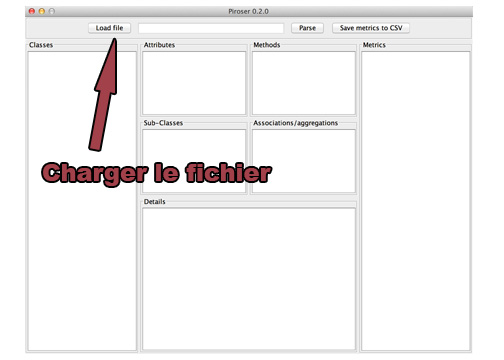
\includegraphics[width=\textwidth]{load_file.jpg}
\caption{\label{fig:load_file}Charger un fichier}
\end{figure}

\begin{figure}
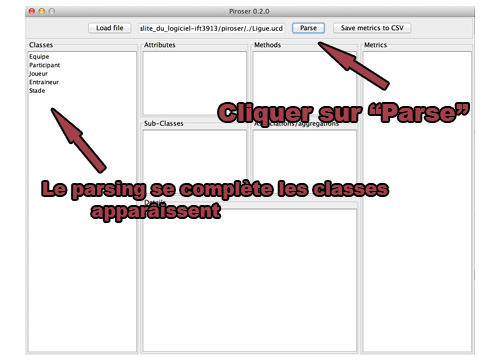
\includegraphics[width=\textwidth]{parsing.jpg}
\caption{\label{fig:parse}Parser le fichier}
\end{figure}

\begin{figure}
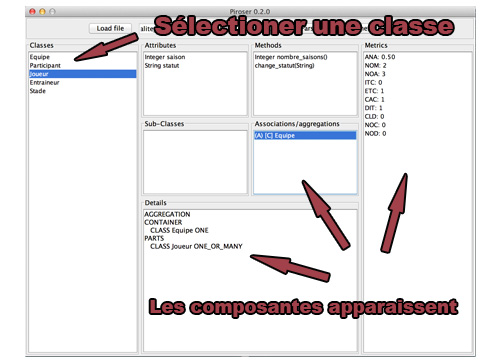
\includegraphics[width=\textwidth]{composantes.jpg}
\caption{\label{fig:view}Visualiser les composantes}
\end{figure}

\subsection{Visualisation des définitions}
Pour visualiser les définitions des acronymes de chaque métrique, il suffi de la sélectionner tel que vu à la figure \ref{fig:definitions}.

\begin{figure}
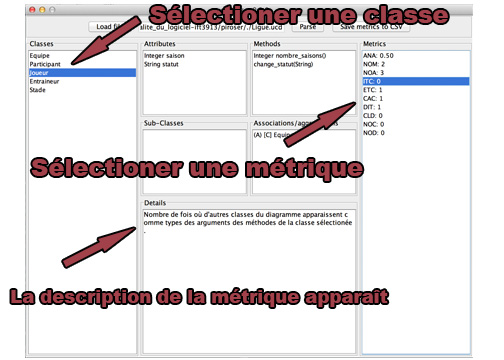
\includegraphics[width=\textwidth]{metrique.jpg}
\caption{\label{fig:definitions}Définitions des métriques}
\end{figure}


\subsection{Génération du CSV}

La génération du CSV se fait en cliquant sur le bouton \texttt{Save metrics to CSV}. Il faudra choisir un emplacement et un nom de fichier. Si le fichier ne se termine pas par \texttt{.csv}, le programme imposera cette extension. Un message de complétion s'affichera s'il n'y a pas eut d'erreurs tel qu'à la figure \ref{fig:save}.

\begin{figure}
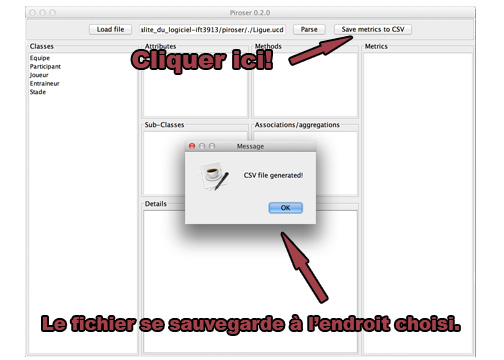
\includegraphics[width=\textwidth]{save.jpg}
\caption{\label{fig:save}Sauvegarde du fichier CSV}
\end{figure}

\end{document}